\documentclass[../thesis.tex]{subfiles}
\section{Contagion on the Model}

Now that the groundwork has been layed down, we can focus on the object of our inquiry: demand shocks and price contagions. As equation (\ref{local_p_comp}) shows, price contagion depends, via $P(\matr{Y})$, on the matrix $(2\I + \G)^{-1}$ which we can define as the ``bargaining power'' matrix, since it allocates the excess revenues, $\Delta_t$, among providers in the network. For example, in the case of a positive demand shock and an increase in the local price of electricity of a given node, the excess demand will be partially absorbed by all other nodes in the network which, in turn, causes a contagion of local price hikes. Hence, the spread of the price hikes depends on the bargaining power of nodes in the matrix. Sticking with our example, if $X_{i, t}$ increases suddenly, $\Delta^{(i, j)}_t$ increases, and the cross-border prices across the network increase by
\begin{equation*}
  (2\I + \G)^{-1}_{(k, l), (i, j)}
\end{equation*}

This implies that a provider with a stronger bargaining position reacts more strongly to price changes, captures higher revenue, which leads to higher prices in the local market. Intuitively it also follows that a denser network, which results in a more equal distribution of bargaining power, leads to lower revenues for providers and lower price hikes. To formalize this, consider the entry $(i, j)$ in $P(\Y_t)$,

\begin{equation*}
  P^{(i, j)}_t = \frac{\sum_{(l, m) \in E} \Delta^{(l, m)}_t \  (2\I + \G)^{-1}_{(i, j), (l, m)}}{Y^{(i, j)}_t},
\end{equation*}

where $\sum_{(l, m) \in E}$ is a summation over the row $(i, j)$ of $(2\I + \G)^{-1}$. Now assume there is some demand shock in a node $k$. We would like to understand the effect this has on prices today, $P^{(i, j)}_t$, and tomorrow, $P^{(i, j)}_{t+1}$. To do so we can first note that the current traded quantity between the two nodes $i$ and $j$, $Y^{(i, j)}_t$, is not affected by a change in $X_{k, t}$ since it will only affect current prices and future quantities between $i$ and $j$ ($X_{k, t} \rightarrow P^{(i, j)}_{t} \rightarrow p_{i, t} \rightarrow X_{i, t+1}$), hence $\partial Y^{(i, j)}_t / \partial X_{k, t} = 0$. This is of course not true for $Y^{(i, j)}_{t+1}$. Then,

\begin{equation}
  \begin{split}
    \frac{\partial P^{(i, j)}_{t}}{\partial X_{k, t}} &= \frac{1}{Y^{(i, j)}_t} \left( p_{k, t} \  \sum_{(k, m) \in E} (2\I + \G)^{-1}_{(i, j), (k, m)} - p_{k, t} \  \sum_{(l, k) \in E} (2\I + \G)^{-1}_{(i, j), (l, k)} \right) \\
    &= \frac{p_{k, t}}{Y^{(i, j)}_t} \underbrace{\left(\sum_{(k, m) \in E} (2\I + \G)^{-1}_{(i, j), (k, m)} -  \sum_{(l, k) \in E} (2\I + \G)^{-1}_{(i, j), (l, k)} \right)}_{\text{influence of $k$ on the network}}
  \end{split}
\end{equation}

This influence value gives a first order approximation of the effect on the network of a demand shock in a given node. In Figure \ref{fig:influence} I plotted the influence of each node on different graphs that will be used in the simulation. It is wise to stop here with the analytical work given the complex behavior of $\partial P^{(i, j)}_{t + 1} / \partial X_{k, t}$, hence in the next section I will look at contagion by picking some simple examples, working out the core structure and influence analytically and then simulate the systems' behavior.

\begin{figure}[H]
  \centering
  % First row
  \begin{subfigure}[t]{.4\textwidth}
    \centering
    \includegraphics[width=\linewidth]{\bargpath/line.pdf}
    \caption{On a path graph} \label{fig:linepower}
  \end{subfigure}
  \hfill
  \begin{subfigure}[t]{.4\textwidth}
    \centering
    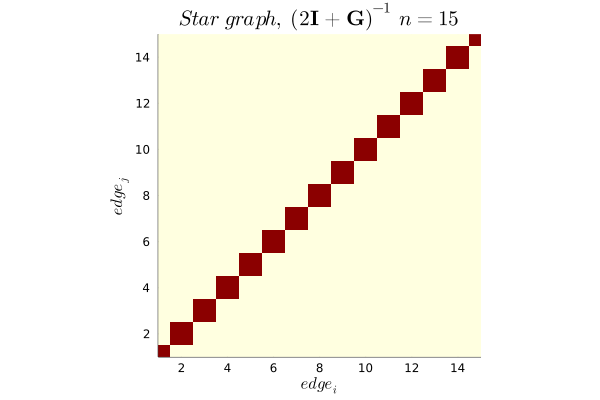
\includegraphics[width=\linewidth]{\bargpath/star.pdf}
    \caption{On a star graph} \label{fig:starpower}
  \end{subfigure}


  \medskip

  % Second row
  \centering
  \begin{subfigure}[t]{.4\textwidth}
    \centering
    \includegraphics[width=\linewidth]{\bargpath/binarytree.pdf}
    \caption{On a binary tree} \label{fig:btreepower}
  \end{subfigure}
  \caption{Network influence} \label{fig:influence}
\end{figure}

\subsection{Two providers}

\subfile{sections/examples/twoproviders.tex}

\subsection{Star and Path}

\subfile{sections/examples/star.tex}

\subsection{Contagion simulation}

A more comprehensive view is given in Figure (\ref{fig:blackout}). Let the standard deviation of the influence of each node on the network, namely

\begin{equation*}
  \rho(\mathcal{A}) = \sqrt{\Var \left(\sum_{(k, m) \in E} (2\I + \G)^{-1}_{(i, j), (k, m)} -  \sum_{(l, k) \in E} (2\I + \G)^{-1}_{(i, j), (l, k)} \right)},
\end{equation*}

be the incoherence of a graph. Intuitively, the bigger and denser the graph, the lower $\rho(\mathcal{A})$. This can be seen in Figure (\ref{fig:incoherence}) where I plot $\rho$ for star, path, and binary graphs. If $n = 3$, the graphs are equivalent and the influence is $1$ for the central node and $0.5$ for the peripheral nodes. Hence, for each,

\begin{equation*}
  \rho = \sqrt{\frac{\left(1 - \frac{2}{3}\right)^2 + 2 \  \left(\frac{1}{2} - \frac{2}{3}\right)^2}{3 - 1}} \approx 2.89.
\end{equation*}

As the number of nodes increases $\rho$ clearly decreases.

\begin{figure}[H]
  \centering
  \includegraphics[width = \textwidth]{\plotpath/blackouts/rhos.pdf}
  \caption{$\rho$ for different graphs and sizes} \label{fig:incoherence}
\end{figure}

Then we can simulate the average blackout, $ \frac{\sum_{t \geq \tau, i} X_{i, t}}{(T - \tau) \  n}$, after a given shock for different network structures. Figure (\ref{fig:blackout}) shows how the size of the blackout is decreasing in graph incoherence.

\begin{figure}[H]
  \centering
  \includegraphics[width = \textwidth]{\plotpath/blackouts/blackoutsim.pdf}
  \caption{Simulation} \label{fig:blackout}
\end{figure}